\documentclass{standalone}
\usepackage{tikz}
\usetikzlibrary{patterns, positioning}
\usepackage[sfdefault]{ClearSans} %% option 'sfdefault' activates Clear Sans as the default text font
\usepackage[T1]{fontenc}

\begin{document}
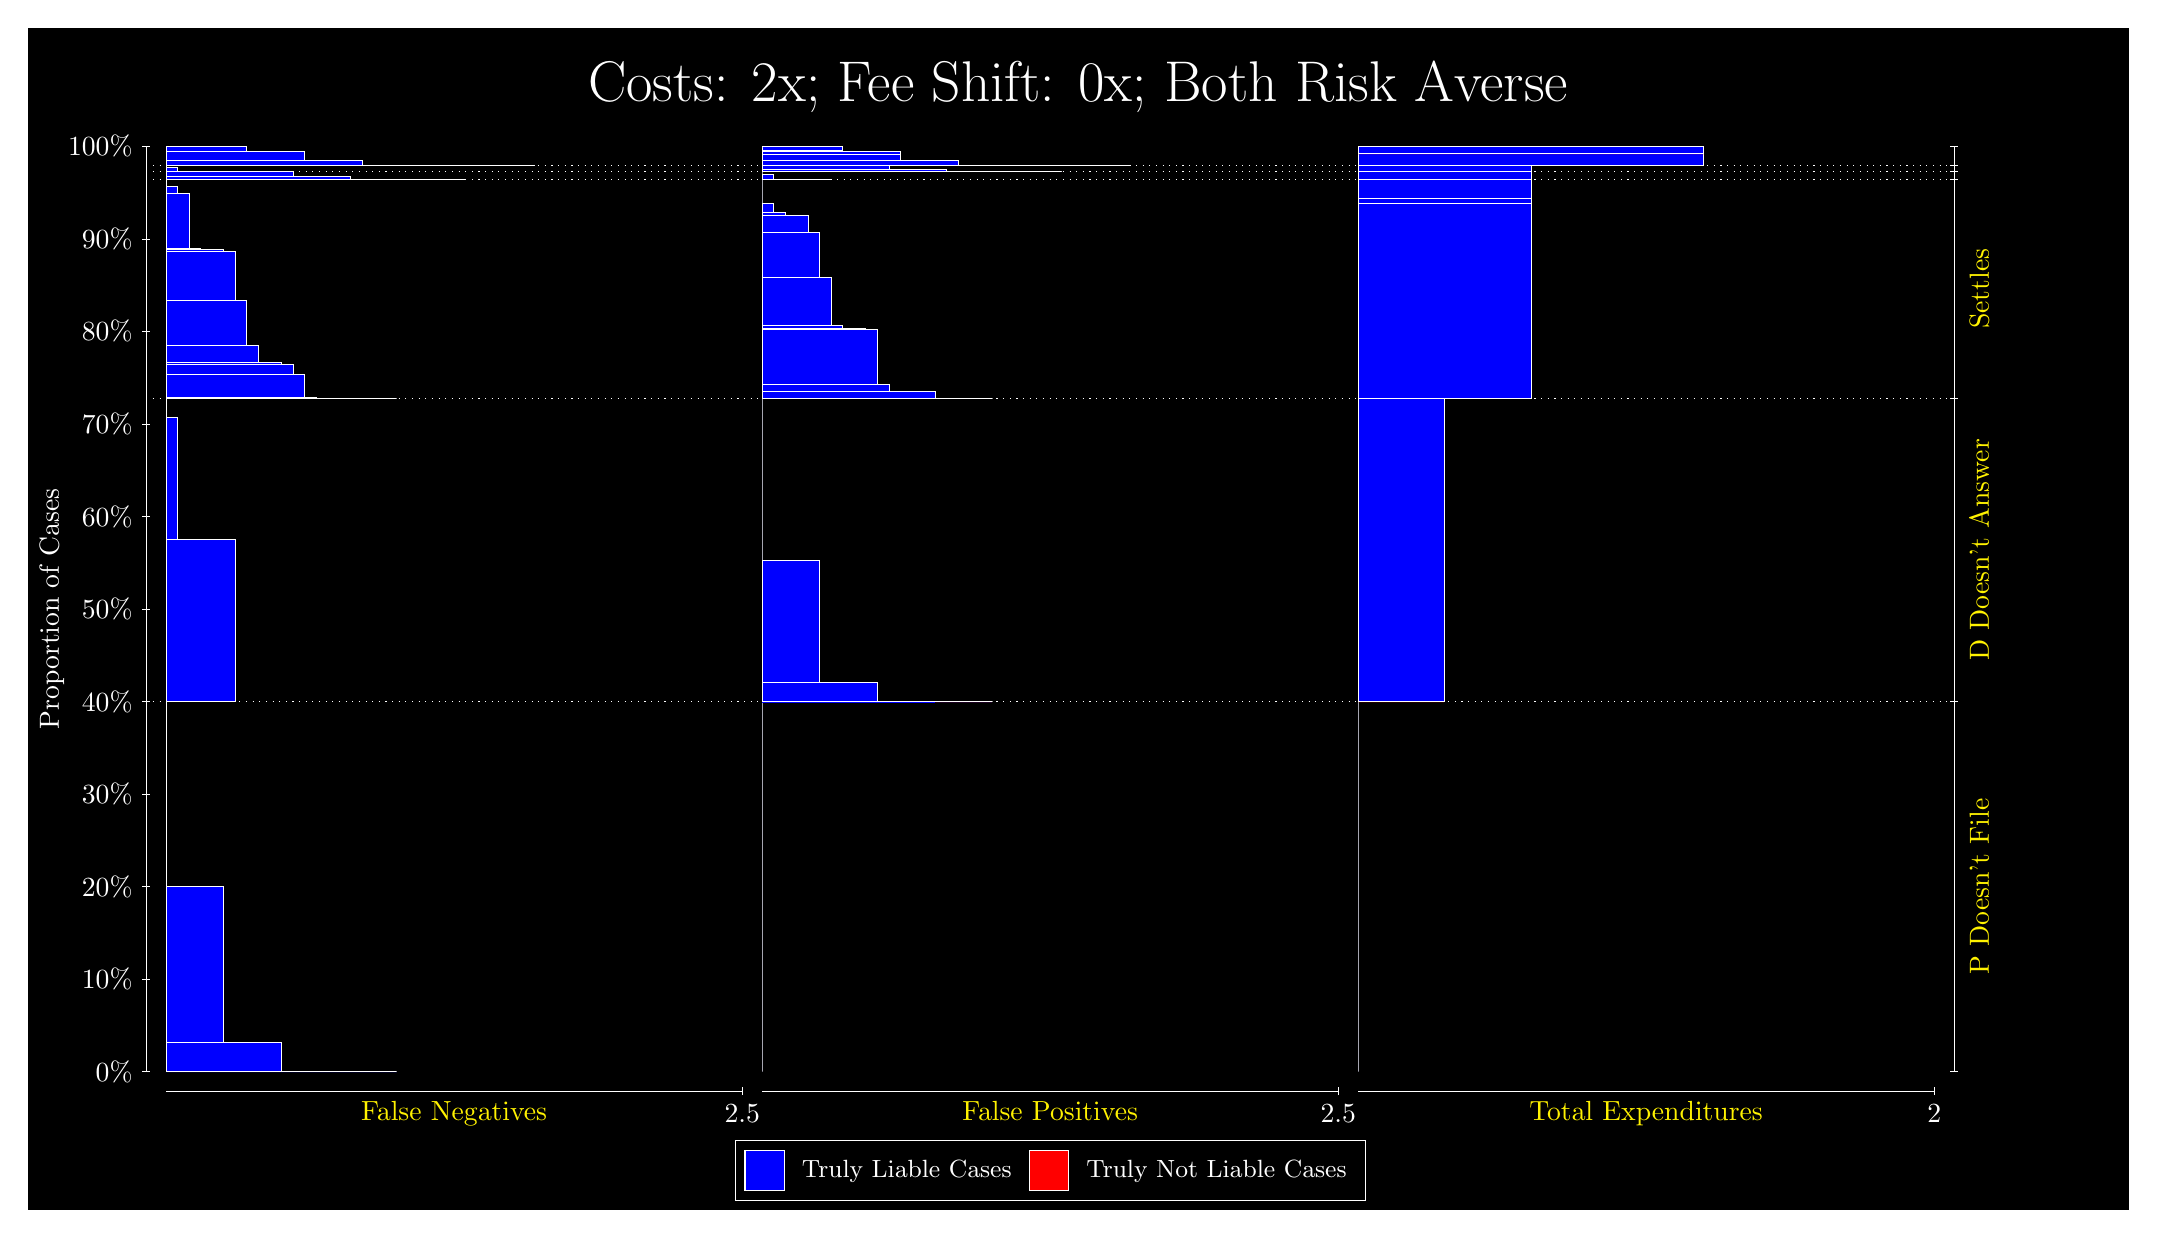
\begin{tikzpicture}
\draw[fill=black] (0,0) rectangle (26.667,15);
\draw[text=white] (0,13.5) rectangle (26.667,15) node[midway] {\huge Costs: 2x; Fee Shift: 0x; Both Risk Averse};
\draw[white, very thin] (1.5,1.75) -- (1.5,13.5);
\node[rotate=90, text=white, anchor=center] at (0.3, 7.625) {Proportion of Cases};
\draw[white, very thin] (1.45,1.75) -- (1.55,1.75);
\node[text=white, anchor=east] at (1.45, 1.75) {0\%};
\draw[white, very thin] (1.45,2.925) -- (1.55,2.925);
\node[text=white, anchor=east] at (1.45, 2.925) {10\%};
\draw[white, very thin] (1.45,4.1) -- (1.55,4.1);
\node[text=white, anchor=east] at (1.45, 4.1) {20\%};
\draw[white, very thin] (1.45,5.275) -- (1.55,5.275);
\node[text=white, anchor=east] at (1.45, 5.275) {30\%};
\draw[white, very thin] (1.45,6.45) -- (1.55,6.45);
\node[text=white, anchor=east] at (1.45, 6.45) {40\%};
\draw[white, very thin] (1.45,7.625) -- (1.55,7.625);
\node[text=white, anchor=east] at (1.45, 7.625) {50\%};
\draw[white, very thin] (1.45,8.8) -- (1.55,8.8);
\node[text=white, anchor=east] at (1.45, 8.8) {60\%};
\draw[white, very thin] (1.45,9.975) -- (1.55,9.975);
\node[text=white, anchor=east] at (1.45, 9.975) {70\%};
\draw[white, very thin] (1.45,11.15) -- (1.55,11.15);
\node[text=white, anchor=east] at (1.45, 11.15) {80\%};
\draw[white, very thin] (1.45,12.325) -- (1.55,12.325);
\node[text=white, anchor=east] at (1.45, 12.325) {90\%};
\draw[white, very thin] (1.45,13.5) -- (1.55,13.5);
\node[text=white, anchor=east] at (1.45, 13.5) {100\%};

\draw[white, very thin] (24.457,1.75) -- (24.457,13.5);
\draw[white, very thin] (24.407,1.75) -- (24.507,1.75);
\node[anchor=west] at (24.407, 1.75) {};
\draw[white, very thin] (24.407,6.4489) -- (24.507,6.4489);
\node[anchor=west] at (24.407, 6.4489) {};
\draw[white, very thin] (24.407,10.3) -- (24.507,10.3);
\node[anchor=west] at (24.407, 10.3) {};
\draw[white, very thin] (24.407,13.084) -- (24.507,13.084);
\node[anchor=west] at (24.407, 13.084) {};
\draw[white, very thin] (24.407,13.185) -- (24.507,13.185);
\node[anchor=west] at (24.407, 13.185) {};
\draw[white, very thin] (24.407,13.26) -- (24.507,13.26);
\node[anchor=west] at (24.407, 13.26) {};
\draw[white, very thin] (24.407,13.5) -- (24.507,13.5);
\node[anchor=west] at (24.407, 13.5) {};

\draw[white, very thin, fill=blue] (1.75,1.75) rectangle (4.6775,1.75);
\draw[white, very thin, fill=blue] (1.75,1.75) rectangle (3.9457,1.7532);
\draw[white, very thin, fill=blue] (1.75,1.7532) rectangle (3.2138,2.126);
\draw[white, very thin, fill=blue] (1.75,2.126) rectangle (2.4819,4.1027);
\draw[white, very thin, fill=red] (1.75,4.1027) rectangle (1.75,4.1027);
\draw[white, very thin, fill=blue] (1.75,4.1027) rectangle (1.75,6.4489);
\draw[white, very thin, fill=blue] (1.75,6.4489) rectangle (2.6283,8.5056);
\draw[white, very thin, fill=blue] (1.75,8.5056) rectangle (1.8964,10.061);
\draw[white, very thin, fill=red] (1.75,10.061) rectangle (1.75,10.061);
\draw[white, very thin, fill=blue] (1.75,10.061) rectangle (1.75,10.3);
\draw[white, very thin, fill=blue] (1.75,10.3) rectangle (4.6775,10.3);
\draw[white, very thin, fill=blue] (1.75,10.3) rectangle (4.3848,10.3);
\draw[white, very thin, fill=blue] (1.75,10.3) rectangle (4.092,10.301);
\draw[white, very thin, fill=blue] (1.75,10.301) rectangle (3.9457,10.301);
\draw[white, very thin, fill=blue] (1.75,10.301) rectangle (3.6529,10.312);
\draw[white, very thin, fill=blue] (1.75,10.312) rectangle (3.5065,10.603);
\draw[white, very thin, fill=blue] (1.75,10.603) rectangle (3.3602,10.727);
\draw[white, very thin, fill=blue] (1.75,10.727) rectangle (3.2138,10.76);
\draw[white, very thin, fill=blue] (1.75,10.76) rectangle (2.921,10.979);
\draw[white, very thin, fill=blue] (1.75,10.979) rectangle (2.7746,11.547);
\draw[white, very thin, fill=blue] (1.75,11.547) rectangle (2.6283,12.161);
\draw[white, very thin, fill=blue] (1.75,12.161) rectangle (2.4819,12.194);
\draw[white, very thin, fill=blue] (1.75,12.194) rectangle (2.1891,12.206);
\draw[white, very thin, fill=blue] (1.75,12.206) rectangle (2.0428,12.902);
\draw[white, very thin, fill=blue] (1.75,12.902) rectangle (1.8964,12.993);
\draw[white, very thin, fill=red] (1.75,12.993) rectangle (1.75,12.993);
\draw[white, very thin, fill=blue] (1.75,12.993) rectangle (1.75,13.084);
\draw[white, very thin, fill=blue] (1.75,13.084) rectangle (5.5558,13.084);
\draw[white, very thin, fill=blue] (1.75,13.084) rectangle (4.8239,13.084);
\draw[white, very thin, fill=blue] (1.75,13.084) rectangle (4.092,13.122);
\draw[white, very thin, fill=blue] (1.75,13.122) rectangle (3.3602,13.183);
\draw[white, very thin, fill=blue] (1.75,13.183) rectangle (2.6283,13.185);
\draw[white, very thin, fill=red] (1.75,13.185) rectangle (1.75,13.185);
\draw[white, very thin, fill=blue] (1.75,13.185) rectangle (2.6283,13.186);
\draw[white, very thin, fill=blue] (1.75,13.186) rectangle (1.8964,13.232);
\draw[white, very thin, fill=red] (1.75,13.232) rectangle (1.75,13.232);
\draw[white, very thin, fill=blue] (1.75,13.232) rectangle (1.75,13.26);
\draw[white, very thin, fill=blue] (1.75,13.26) rectangle (6.4341,13.26);
\draw[white, very thin, fill=blue] (1.75,13.26) rectangle (5.7022,13.26);
\draw[white, very thin, fill=blue] (1.75,13.26) rectangle (4.9703,13.263);
\draw[white, very thin, fill=blue] (1.75,13.263) rectangle (4.2384,13.319);
\draw[white, very thin, fill=blue] (1.75,13.319) rectangle (3.5065,13.44);
\draw[white, very thin, fill=blue] (1.75,13.44) rectangle (2.7746,13.496);
\draw[white, very thin, fill=blue] (1.75,13.496) rectangle (2.0428,13.5);
\draw[white, very thin, fill=red] (1.75,13.5) rectangle (1.75,13.5);
\draw[white, very thin, fill=blue] (1.75,13.5) rectangle (1.75,13.5);
\draw[white, very thin, fill=red] (9.3189,1.75) rectangle (9.3189,1.75);
\draw[white, very thin, fill=blue] (9.3189,1.75) rectangle (9.3189,6.4489);
\draw[white, very thin, fill=red] (9.3189,6.4489) rectangle (12.246,6.4489);
\draw[white, very thin, fill=blue] (9.3189,6.4489) rectangle (12.246,6.4489);
\draw[white, very thin, fill=blue] (9.3189,6.4489) rectangle (11.515,6.4493);
\draw[white, very thin, fill=blue] (9.3189,6.4493) rectangle (10.783,6.6885);
\draw[white, very thin, fill=blue] (9.3189,6.6885) rectangle (10.051,8.2436);
\draw[white, very thin, fill=blue] (9.3189,8.2436) rectangle (9.3189,10.3);
\draw[white, very thin, fill=red] (9.3189,10.3) rectangle (12.246,10.3);
\draw[white, very thin, fill=blue] (9.3189,10.3) rectangle (12.246,10.3);
\draw[white, very thin, fill=red] (9.3189,10.3) rectangle (11.661,10.3);
\draw[white, very thin, fill=blue] (9.3189,10.3) rectangle (11.661,10.301);
\draw[white, very thin, fill=blue] (9.3189,10.301) rectangle (11.515,10.391);
\draw[white, very thin, fill=red] (9.3189,10.391) rectangle (11.368,10.391);
\draw[white, very thin, fill=blue] (9.3189,10.391) rectangle (11.368,10.391);
\draw[white, very thin, fill=red] (9.3189,10.391) rectangle (11.075,10.391);
\draw[white, very thin, fill=blue] (9.3189,10.391) rectangle (11.075,10.392);
\draw[white, very thin, fill=blue] (9.3189,10.392) rectangle (10.929,10.482);
\draw[white, very thin, fill=blue] (9.3189,10.482) rectangle (10.783,11.178);
\draw[white, very thin, fill=blue] (9.3189,11.178) rectangle (10.636,11.19);
\draw[white, very thin, fill=blue] (9.3189,11.19) rectangle (10.344,11.223);
\draw[white, very thin, fill=blue] (9.3189,11.223) rectangle (10.197,11.838);
\draw[white, very thin, fill=blue] (9.3189,11.838) rectangle (10.051,12.405);
\draw[white, very thin, fill=blue] (9.3189,12.405) rectangle (9.9044,12.624);
\draw[white, very thin, fill=blue] (9.3189,12.624) rectangle (9.6116,12.657);
\draw[white, very thin, fill=blue] (9.3189,12.657) rectangle (9.4652,12.781);
\draw[white, very thin, fill=blue] (9.3189,12.781) rectangle (9.3189,13.084);
\draw[white, very thin, fill=red] (9.3189,13.084) rectangle (10.197,13.084);
\draw[white, very thin, fill=blue] (9.3189,13.084) rectangle (10.197,13.086);
\draw[white, very thin, fill=blue] (9.3189,13.086) rectangle (9.4652,13.147);
\draw[white, very thin, fill=blue] (9.3189,13.147) rectangle (9.3189,13.185);
\draw[white, very thin, fill=red] (9.3189,13.185) rectangle (13.125,13.185);
\draw[white, very thin, fill=blue] (9.3189,13.185) rectangle (13.125,13.185);
\draw[white, very thin, fill=blue] (9.3189,13.185) rectangle (12.393,13.185);
\draw[white, very thin, fill=blue] (9.3189,13.185) rectangle (11.661,13.213);
\draw[white, very thin, fill=blue] (9.3189,13.213) rectangle (10.929,13.259);
\draw[white, very thin, fill=blue] (9.3189,13.259) rectangle (10.197,13.26);
\draw[white, very thin, fill=red] (9.3189,13.26) rectangle (14.003,13.26);
\draw[white, very thin, fill=blue] (9.3189,13.26) rectangle (14.003,13.26);
\draw[white, very thin, fill=red] (9.3189,13.26) rectangle (13.271,13.26);
\draw[white, very thin, fill=blue] (9.3189,13.26) rectangle (13.271,13.26);
\draw[white, very thin, fill=red] (9.3189,13.26) rectangle (12.539,13.26);
\draw[white, very thin, fill=blue] (9.3189,13.26) rectangle (12.539,13.264);
\draw[white, very thin, fill=blue] (9.3189,13.264) rectangle (11.807,13.32);
\draw[white, very thin, fill=red] (9.3189,13.32) rectangle (11.807,13.32);
\draw[white, very thin, fill=blue] (9.3189,13.32) rectangle (11.807,13.32);
\draw[white, very thin, fill=blue] (9.3189,13.32) rectangle (11.075,13.397);
\draw[white, very thin, fill=red] (9.3189,13.397) rectangle (11.075,13.397);
\draw[white, very thin, fill=blue] (9.3189,13.397) rectangle (11.075,13.441);
\draw[white, very thin, fill=blue] (9.3189,13.441) rectangle (10.344,13.451);
\draw[white, very thin, fill=blue] (9.3189,13.451) rectangle (10.344,13.497);
\draw[white, very thin, fill=blue] (9.3189,13.497) rectangle (9.6116,13.497);
\draw[white, very thin, fill=blue] (9.3189,13.497) rectangle (9.6116,13.5);
\draw[white, very thin, fill=blue] (9.3189,13.5) rectangle (9.3189,13.5);
\draw[white, very thin, fill=red] (16.888,1.75) rectangle (16.888,1.75);
\draw[white, very thin, fill=blue] (16.888,1.75) rectangle (16.888,6.4489);
\draw[white, very thin, fill=red] (16.888,6.4489) rectangle (17.986,6.4489);
\draw[white, very thin, fill=blue] (16.888,6.4489) rectangle (17.986,10.3);
\draw[white, very thin, fill=red] (16.888,10.3) rectangle (19.083,10.3);
\draw[white, very thin, fill=blue] (16.888,10.3) rectangle (19.083,12.775);
\draw[white, very thin, fill=red] (16.888,12.775) rectangle (19.083,12.775);
\draw[white, very thin, fill=blue] (16.888,12.775) rectangle (19.083,12.842);
\draw[white, very thin, fill=red] (16.888,12.842) rectangle (19.083,12.842);
\draw[white, very thin, fill=blue] (16.888,12.842) rectangle (19.083,13.084);
\draw[white, very thin, fill=red] (16.888,13.084) rectangle (19.083,13.084);
\draw[white, very thin, fill=blue] (16.888,13.084) rectangle (19.083,13.185);
\draw[white, very thin, fill=red] (16.888,13.185) rectangle (19.083,13.185);
\draw[white, very thin, fill=blue] (16.888,13.185) rectangle (19.083,13.26);
\draw[white, very thin, fill=red] (16.888,13.26) rectangle (21.279,13.26);
\draw[white, very thin, fill=blue] (16.888,13.26) rectangle (21.279,13.406);
\draw[white, very thin, fill=red] (16.888,13.406) rectangle (21.279,13.406);
\draw[white, very thin, fill=blue] (16.888,13.406) rectangle (21.279,13.5);
\draw[white, dotted] (1.5,6.4489) -- (24.457,6.4489);
\draw[white, dotted] (1.5,10.3) -- (24.457,10.3);
\draw[white, dotted] (1.5,13.084) -- (24.457,13.084);
\draw[white, dotted] (1.5,13.185) -- (24.457,13.185);
\draw[white, dotted] (1.5,13.26) -- (24.457,13.26);
\draw[white, very thin] (1.75,1.5) -- (9.0689,1.5);
\node[text=yellow, anchor=north] at (5.4094, 1.5) {False Negatives};
\draw[white, very thin] (9.0689,1.45) -- (9.0689,1.55);
\node[text=white, anchor=north] at (9.0689, 1.45) {2.5};

\draw[white, very thin] (9.3189,1.5) -- (16.638,1.5);
\node[text=yellow, anchor=north] at (12.978, 1.5) {False Positives};
\draw[white, very thin] (16.638,1.45) -- (16.638,1.55);
\node[text=white, anchor=north] at (16.638, 1.45) {2.5};

\draw[white, very thin] (16.888,1.5) -- (24.207,1.5);
\node[text=yellow, anchor=north] at (20.547, 1.5) {Total Expenditures};
\draw[white, very thin] (24.207,1.45) -- (24.207,1.55);
\node[text=white, anchor=north] at (24.207, 1.45) {2};

\node[text=yellow, centered, rotate=90] at (24.777, 4.0995) {P Doesn't File};
\node[text=yellow, centered, rotate=90] at (24.777, 8.3746) {D Doesn't Answer};
\node[text=yellow, centered, rotate=90] at (24.777, 11.692) {Settles};




\draw (12.978300999999998,1.5) node[draw=none] (baseCoordinate) {};
\begin{scope}[align=center]
        \matrix[scale=0.5, draw=white, below=0.5cm of baseCoordinate, nodes={draw}, column sep=0.1cm]{
            \node[rectangle, draw, minimum width=0.5cm, minimum height=0.5cm, fill=blue] {}; &
            \node[draw=none, font=\small, text=white] (B) {Truly Liable Cases}; &
            \node[rectangle, draw, minimum width=0.5cm, minimum height=0.5cm, fill=red] {}; &
            \node[draw=none, font=\small, text=white] (B) {Truly Not Liable Cases}; \\
            };
\end{scope}

\end{tikzpicture}
\end{document}